%!TEX root=../document.tex
\section{Corba Allgemein (Overview)}
\label{sec:Corba Allgemein (Overview)}


	\subsection{Was ist CORBA \cite{omniOrb} \cite{corbaWiki}}

	CORBA (\textbf{C}ommon \textbf{O}bject \textbf{R}equest \textbf{B}roker \textbf{A}rchitecture) vereinfacht das Erstellen verteilter Anwendungen und soll das Aufrufen externer Methoden ermöglichen bzw. vereinfachen.
	
	Der große Vorteil von CORBA ist die Plattformunabhängigkeit und ist somit, im Gegensatz zu anderen Umsetzungen, nicht an eine Spezielle Umgebung gebunden.
	CORBA setzt darauf, dass die Hersteller bzw. Communities, auf der Grundlage der Spezifikation eigene Object-Request-Broker Implementierungen erstellen und weiter verbessern. Deshalb können Hersteller Ihre Implementierungen für mehrere Programmiersprachen und auch unterschiedliche Betriebssysteme anbieten.
	
	Die gemeinsame Spezifikation ermöglicht dann die Kommunikation von Anwendungen untereinander, die mit unterschiedlichen Programmiersprachen erstellt worden sind, verschiedene ORBs nutzen und auf verschiedenen Betriebssystemen und Hardwareumgebungen laufen können.
	
		\subsection{Überblick CORBA \cite{omniOrb} \cite{corbaWiki}}
		Mithilfe von der \textit{Interface Definition Language (IDL)} können formale Spezifikationen der Schnittstellen (Datentypen und Methodensignaturen), die ein Objekt für remote oder lokale Zugriffe zur Verfügung stellen, umgesetzt werden.
		
		Damit das ganze Prinzip funktioniert müssen diese definierten Schnittstellen (in Java Interfaces) für alle anderen Programmiersprachen umgesetzt werden.
		Dafür müssen diese nun von dem entsprechenden IDL-Compiler in äquivalente Beschreibungen der Schnittstellen kompiliert werden.
		
		Ebenfalls wird Quellcode, welcher zu der benutzten ORB-Implementierung passt, erstellt. Deiser Quelltext enthält, wie wir bereits von \textit{Remote Method Invocation} kennen, die Implementierung des Skelletons bzw. Stubs für Callback am Client usw. Durch dieses \textit{Vermittler-Pattern} erscheinen remote Aufrufe fast so einfach wie lokale Aufrufe und verbirgt somit die Komplexität der damit verbundenen Netzwerkkommunikation.
		
		Bei unserem Beispiel verwenden wie die Java Implementierung \textbf{\texttt{jackorb \cite{jackorb}}} und die C++/Python Implementierung \textbf{\texttt{omniOrb \cite{omniOrb}}}
		
		\clearpage
		
		\subsection{Unterschied zu RMI \cite{corbaPDF}}
		Der große (offensichtliche) Unterschied ist die Tatsache, dass CORBA Plattformunabhängig (\texttt{Common}) arbeitet, wobei RMI eine Java Implementierung ist, welche ausschließlich unter Java bzw in Java Umgebungen läuft. 
		Aus diesem Grund können wir in RMI normale Java Interfaces benutzen. Beispielweise muss der Client, um von einem Remote Object eine Methode invoken zu können, muss zuerst die Struktur mithilfe eines entsprechendem Interfaces bekannt sein. Bei CORBA ist dies ähnlich jedoch muessen diese "Interfaces/Header Files" mithilfe der IDL (Interface Definition Language) kompiliert werden, damit jede unterstützte Programmiersprache auf jene Interfaces zugreifen kann.
		
		\subsection{CORBA im Detail \cite{corbaPDF}}
		\begin{figure}[!h]
			\begin{center}
				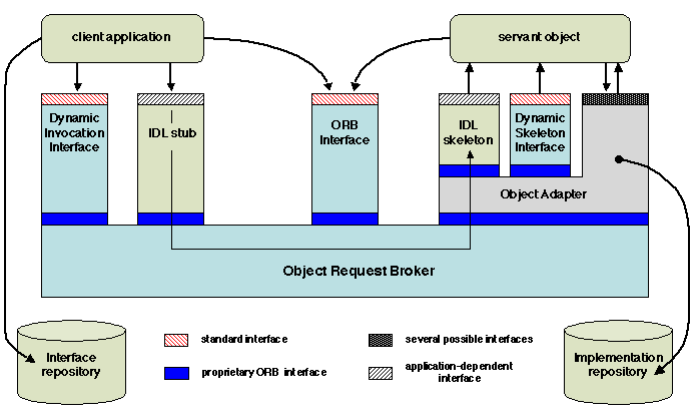
\includegraphics[width=0.6\linewidth]{images/corbaArchitektur.png}
				\caption{CORBA - Architektur \cite{corbaArchitektur}}
				\label{Decorator Pattern - Klassen Diagramm}
			\end{center}
		\end{figure}
		
			\subsubsection{Object Request Broker (ORB) \cite{corbaPDF}}
			Am besten laesst sich ein ORB mit einem Datenbus vergleichen. Wir haben beispielsweise eine CPU oder andere HW, welche mit bestimmter anderen Hardware kommunizieren will. Über einen Datenbus laesst sich dies gut realisieren. Ein ORB funktioniert ähnlich.
			
			Sowhol die Client Seite (stub) als auch der Server (OA) haben Zugriff auf diesen ORB. Der Object Request Broker ist zuständig für jegliche Kommunikation zwischen dem Object Adapter und dem entsprechendem stub am Client.
			
			Ebenfalls werden sämtliche Services (NameService, Mapper, Convertior usw.) über den ORB gesteuert und angesprochen.
			
			\subsubsection{Interface Definition Language \cite{corbaPDF} \cite{omgCorba}}
			IDL ist einer der wichtigsten Komponenten im Cyklus von CORBA. Da wir nicht wie in RMI nur innerhalb unserer JVM sind, müssen wir uns irgendwie überlegen, wie unsere Klassen bzw. Methoden Strukturen für möglichst viele andere Programmiersprachen lesbar bzw. verständlich darzustellen.
			Die Lösung ist der IDL Compiler, welcher direkt von CORBA mitgeliefert wird.
			
			Natürlich kann das Mapping nur erfolgen wenn für die gewünschte Programmiersprache eine entsprechende Implementierung existiert. Das Mapping gitb an wie ein Interface in IDL mit der Implementation der Programmiersprache zusammenhaengt.
			
			\begin{itemize}
				\item Descriptive language
				\item Keine Logik / Algorithmen
				\item nur Syntax, Semnatik muss separat angegeben werden
				\item Sprachen spezifisches Mapping für verschiedene Programmiersprachen
				\item IDL - Compiler erzeugt Programm spezifischen Code (stub, skeleton etc.)
				\item Modules declare Namespaces, Value Types for Data Transfer
			\end{itemize}
			
			Ein kurzes, konkretes Beispiel zur Erklärung:
			
			\begin{lstlisting}[style=C++, caption=IDL Example \cite{corbaPDF}]	
			module calculator {
				module common {
					exception CalculatorException {
						string details;
					};
					interface Calculator {
						long add(in long a, in long b);
						long sub(in long a, in long b);
						long mul(in long a, in long b);
						long div(in long a, in long b)
						raises (CalculatorException));
					};
				};
			};
			\end{lstlisting}
			
			\clearpage
			
			\subsubsection{(Protable) Object Adapter ((P)OA)\cite{corbaPDF} \cite{poaWiki}}
			\begin{figure}[!h]
				\begin{center}
					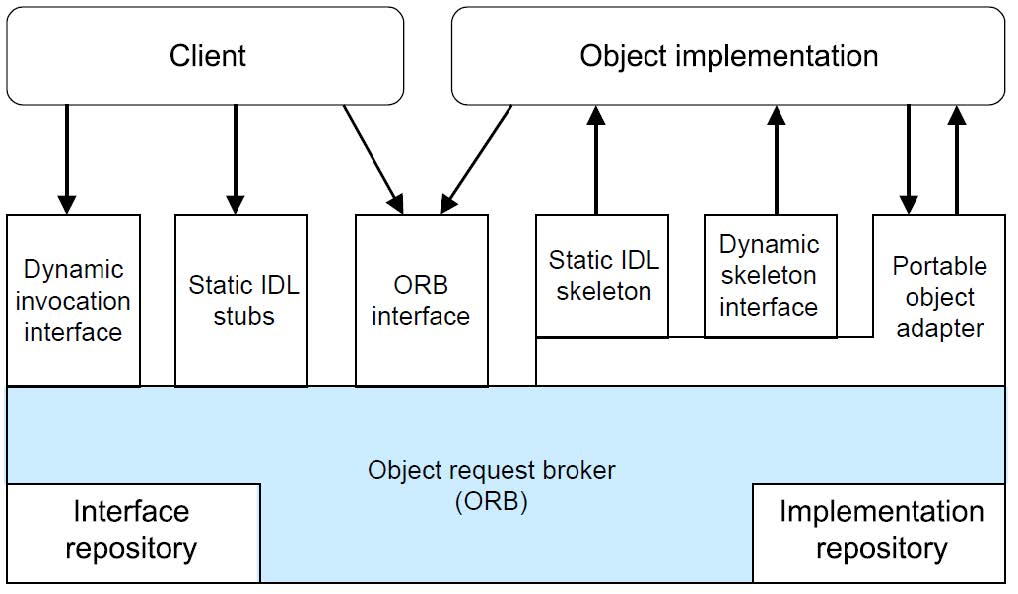
\includegraphics[width=0.4\linewidth]{images/corba.jpg}
					\caption{CORBA POA Managerr \cite{corbaPDF}}
					\label{CORBA POA}
				\end{center}
			\end{figure}
			
			Der POA ist ein wichtiger Ankerpunkt, damit das Prinzip von CORBA funktionieren kann. Der Object Manager, wie der Name schon verrät, verwaltet die Objekte des Servers.\\
			Das bedeutet sobald der ORB versucht ein Objekt zu invoken bzw zu finden kommt der POA ins Spiel. Er hat folgende wichtigen Aufgaben:
				\begin{itemize}
					\item Generation sowie Implementation der Objekt Referenzen
					\item Methoden invokation / Aufruf, Registration von Implementationen
					\item Object activation / deactivation
					\item Falls notwendig bereitstellen des Skeleton am Server
					\item etc.
				\end{itemize}
				
			\subsubsection{POA Manager Factory}
			Damit wir nicht jedes Mal, wenn wir einen neuen POA-Manager instanzieren (\texttt{new POAManager()}), alle dazugehörigen Eigenschaften explicit setzten müssen. Gibt es Abhilfe durch das Factory Pattern) Also verwenden wir die Factory, damit wir unsere Eigenschaften übergeben können, ohne uns darum zu kümmern alle nötigen (korrekten) Eigenschaften jedes Mal erneut zu setzten.\\
			Beispiel:
			\begin{lstlisting}[style=C++, caption=IDL Example \cite{corbaPDF}]	
			.POAManager create_POAManager(in string id, in CORBA::PolicyList policies)
				 raises(ManagerAlreadyExists, CORBA::PolicyError);
			\end{lstlisting}
			\clearpage
	
\section{Vorbereitung \cite{ubuntuCompile}}
Damit wir die \textbf{\texttt{omniOrb \cite{omniOrb}}} bzw \textbf{\texttt{jackorb \cite{jackorb}}} Implementationen verwenden können müssen diese zuerst gebuildet bzw. kompiliert werden.

Der große Vorteil ist, dass das Builden / Kompilieren für die entsprechende Plattform durchgeführt wird und somit auf jeden Fall die optimale Leistung bzw. Effizienz herausgeholt werden kann.

Bei der Kompilierung ist darauf zu achten in welcher Programmiersprache der Programmcode geschrieben wurde und welcher Compiler von dem Programmierer bevorzugt wird.\\

\subsection{Kompilieren von \texttt{omniOrb \cite{omniOrb}}}

\begin{lstlisting}[style=BashInputStyle, caption=Compiling omniOrb \cite{ubuntuConfigure}]
# Binaries for omniOrb
wget omniORB PATH
# !README LESEN!
# Folgende Vorgaenge wurden in der README aufgelistet:
#	mkdir build
#	cd build
#	make
#	make install
# Konfigurieren
# Es wird ein script gestartet, welches berprueft ob das Programm mit der aktuellen Programmumgebung kompatibel
# ist und setzt falls noetig systemspezifische Optionen im Makefile
# Damit ../configure ohne Probleme ablaufen kann muessen alle benoetigten Packages installiert sein
# bsp. gcc usw.
mkdir build
cd build
../configure
# Nun muss make ausgefuehrt werden hierbei wird das vorliegende Makefile hergenommen und demenstprechend gebuildet
# Mit make insall die Installation abschliesen nun sollten alle Variablen gesetzt und alles Kompiliert sein.
make
make install
# Anschliesend sollten wir folgende Directory Struktur haben
# Wobei sich in lib alle notwendigen (fuer die kompilierte Plattform) benoetigten Libraries befinden
# Und im bin/ Ordner werden alle executable Services gespeicchtert, wie beispielsweise der NameService usw.
ls
bin  config.log  config.status  contrib  etc  GNUmakefile  idl  include  lib  mk  src  stub
# Ausfuehren bzw. builden eines Examples
cd src/examples/call_back
ls
GNUmakefile
# Um unser Example zu kompilieren muss wieder das vorliegende Make 
make
ls
cb_client    cb_client.o  cb_server.d  cb_shutdown    GNUmakefile
cb_client.d  cb_server    cb_server.o  cb_shutdown.o
# Nach dem das Kompilieren erfolgreich war koennen alle executables noraml mit ./<name> <param> ausgefuehrt werden

\end{lstlisting}

\clearpage
\subsection{Probleme beim Builden}
Da ich die README nicht \textbf{genau} gelesen habe, wurden mehrere Schritte umständlicher und komplizierter als sie eigentlich sein hätten können.

Theoretisch hätte das Programm auch mit \texttt{apt-get install} funktioniert. Doch unter anderem war es ein Ziel der Übung mithilfe von make / GnuMake ein Programm für die entsprechende Plattform zu kompilieren sowie alle notwendigen Probleme, welche unmittelbar damit verbunden sind zu lösen und festzuhalten.

Der README zufolge wird in \texttt{/build ../configure} und anschlisend \texttt{make / make install} ausgefuehrt wenn dies wie in Punkt 3.1 Kompilieren von omniOrb beschrieben, befolgt wird funktioniert das make ohne weitere Probleme.

Da ich die Examples im falschen Ordner --> \texttt{/-/omniOrb/src/examples} und nicht, wie in der README beschrieben in \texttt{/-/omniOrb/build/src/examples} gebuildet habe sind bei \texttt{make / make install} mehrere Fehler aufgetreten.

Um diese Probleme zu beheben wurden folgende Schritte bzw. Schlupfloecher durchgefuehrt.

Durch den falschen Pfad musste zuerst vor dem \texttt{make} die Datei \texttt{/config/config.mk} bearbeitet und auf die passende Plattform umgeschrieben werden. Da unser debian System nicht aufgelistet war wurde als Ersatz \texttt{i586 linux 2.0} verwendet. Um dies auch den anderen Services welche auf shared libraries zugreifen zu vermitteln musste in den entsprechenden Verzeichnissen ein Sysmbolik Link auf die gewaehlte Plattform gesetzt werden.

Anschliesend konnten die Examples erfolgreich gebuildet und ausgefuehrt werden. Aber nur mit \texttt{Segmentation fault} als warning

\subsection{Probleme beim Ausfuehren}
Beim ausfuehren der kompilierten Programme ist jedeglich ein Fehler aufgetreten:
\begin{lstlisting}[style=BashInputStyle, caption=Problem beim Ausfuehren]
./cb_server
./cb_server: error while loading shared libraries: libomniORB4.so.2: cannot open shared object file: 
No such file or directory
# Dieser Fehler tritt auf wenn der LD_LIBRARY_PATH nicht korrekt gesetzt wurde.
# Um diesen search PATH zu aendern muss wie folgt vorgegangen werden.
LD_LIBRARY_PATH=/home/pkogler/downloads/omniORB-4.2.1/build/
export LD_LIBRARY_PATH
\end{lstlisting}

\clearpage
\section{Ergebnisse}
\label{sec:Ergebnisse}
Um die Aufgabenstellung vollstaendig zu loesen wurde ein example aus \texttt{/build/src/example} genommen und entsprechend umgeschrieben.
In meinem Fall habe ich das call back example aus omniORB genommen. Übernommen wurde die Implementierung des Servers in C++. Der Client wurde von scratch mithilfe der GitHub code Examples \cite{borkoRepo} in Java geschrieben.

Um die Examples korrekt zu builden war fuer den Server ein entsprechendes Makefile und fuer den Client ein build.xml (ant) notwendig. Hierbei wurden die Interfaces mittels \texttt{jacORB / omniORB} kompiliert sowie die jewwiligen Sources generiert, welche fuer eine erfolgreiche Kommunikation zwischen dem Server und dem Client notwendig sind.

\subsection{Die Server Seite C++}
Das bereits bestehende Example call back bietet eine C++ Server implementierung welches es ermoeglicht die  Methoden \texttt{one time(String msg), register(Callback, String msg)} zu invoken und anschliesend wieder unregistern
Das zugehoerige \texttt{idl} File sieht wie folgt aus:
\begin{lstlisting}[style=C++, caption=echo.idl call back]	
#ifndef __ECHO_CALLBACK_IDL__
#define __ECHO_CALLBACK_IDL__

module cb {
	interface CallBack {
		void call_back(in string mesg);
	};
	interface Server {
	// Server calls back to client just once in a
	// recursive call before returning.
	void one_time(in CallBack cb, in string mesg);
	// Server remembers the client's reference, and
	// will call the call-back periodically.  It stops
	// only when shutdown, or a call to the client fails.
	void register(in CallBack cb, in string mesg,
	in unsigned short period_secs);
	// Shuts down the server.
	void shutdown();
	};
};

#endif
\end{lstlisting}

\clearpage

\subsubsection{Makefile des Servers}
Wie bereits beschrieben wird ein Makefile benoetigt um Den server.cc zu builden. Damit alle sources gebuildet werden. Das Makefile beinhaltet Informationen ueber den Pfad von omniOrb, den idl Compiler sowie welche Dateien bzw. Ordner gebuildet werden und welche dementsprechende Regeln zu befolgen sind.
Das Makefile sieht wie folgt aus:
\begin{lstlisting}[style=C++, caption=echo.idl call back]	
CXX             = /usr/bin/g++
CPPFLAGS        = -g -c
LDFLAGS         = -g
OMNI_HOME       = /home/pkogler/downloads/omniORB-4.2.1/
OMNIIDL         = $(OMNI_HOME)/build/bin/omniidl
LIBS            = -lomniORB4 -lomnithread -lomniDynamic4
OBJECTS         = echoSK.o server.o
IDL_DIR         = ../idl
IDL_FILE        = $(IDL_DIR)/echo.idl

all server: $(OBJECTS)
	$(CXX) $(LDFLAGS) -o server server.o echoSK.o $(LIBS)

server.o: server.cc
	$(CXX) $(CPPFLAGS) server.cc -I.

echoSK.o: echoSK.cc echo.hh
	$(CXX) $(CPPFLAGS) echoSK.cc -I.

echoSK.cc: $(IDL_FILE)
	$(OMNIIDL) -bcxx $(IDL_FILE)

run: server
	# Start Naming service with command 'omniNames -start -always' as root
	./server -ORBInitRef NameService=corbaname::localhost

clean clean-up:
rm -rf *.o

\end{lstlisting}


\subsubsection{Ausfuehren des Servers / Ausgabe (Aufrufe) des Clients}
\begin{lstlisting}[style=BashInputStyle, caption=Ausfuehern des Servers]
omniNames -start -always	# Starten des NameService
./server -ORBInitRef NameService=corbaname::localhost
# Ausgabe
IOR:0101------100101010
cb_server: Doing a single call-back: Meine Nachricht Single
cb_server: Starting a new worker thread
cb_server: Lost a client!
cb_server: Worker thread is exiting.
\end{lstlisting}

\clearpage

\subsection{Die Client Seite Java}
Nachdem der Server funktioniert brauchen wir nur noch eine Client Implementation welche die gewuenschten Methoden invoked.
Bei dem Client musste der NameService konfiguriert werden sowie das Callback interface.
Der Client wurde wie folgt umgesetzt:
\begin{lstlisting}[style=Java, caption=Code des Clients \cite{borkoRepo}]
public class Client extends CallBackPOA {
	public static void main(String[] args)  {
		Server echo;
		try {

			/* Erstellen und intialisieren des ORB */
			ORB orb = ORB.init(args, null);

			/* Erhalten des RootContext des angegebenen Namingservices */
			Object o = orb.resolve_initial_references("NameService");
			/* Verwenden von NamingContextExt */
			NamingContextExt rootContext = NamingContextExtHelper.narrow(o);
			/* Angeben des Pfades zum Echo Objekt */
			NameComponent[] name = new NameComponent[2];
			name[0] = new NameComponent("test","my_context");
			name[1] = new NameComponent("Echo", "Object");

			/* Aufloesen der Objektreferenzen  */
			echo = ServerHelper.narrow(rootContext.resolve(name));

			POA root_poa = (POA) orb.resolve_initial_references ("RootPOA");
			root_poa.the_POAManager().activate();
			CallBack ccb = CallBackHelper.narrow (root_poa.servant_to_reference (new Client()));

			echo.one_time(ccb, "Meine Nachricht Single");

			echo.register(ccb, "Meine Nachricht register", period);

			try {
				Thread.sleep(5000);
			} catch (Exception e) {
				e.printStackTrace();
			}

			//System.out.println("Der Server sagt: " + echo.echoString("Hallo Welt!"));

			}       catch (Exception e)     {
				System.err.println("Es ist ein Fehler aufgetreten: " + e.getMessage());
				e.printStackTrace();
			}
		}
	}
	public void call_back(String msg) {
		System.out.println ("Client callback object received a message >" + msg + '<');
	}
}

\end{lstlisting}

\clearpage

\subsubsection{build.xml File fuer den Build}
In dem build File werden wieder alle noetigen Variablen gesetzt welche benoetigt werden um jacorb auszufuehren und alle sources fuer die Implementierung zu generieren.
Das build.xml sieht wie folgt aus:

\begin{lstlisting}[basicstyle=\tiny, style=XML, caption=Code des Clients \cite{borkoRepo}]
<project name="client">
	
	<!-- Setzen aller Variablen -->
	<property name="src.dir" value="src" />
	<property name="build.dir" value="build" />
	<property name="classes.dir" value="${build.dir}/classes" />
	<property name="doc.dir" value="doc" />
	<property name="idl.dir" value="../idl" />
	<property name="gen.dir" value="${build.dir}/generated" />
	<property name="resources.dir" value="resources" />
	<property name="jacorb.dir" value="/home/pkogler/downloads/jacorb-3.7" />
	<property name="tmp.dir" value="${build.dir}/tmp" />
	<property name="host" value="127.0.0.1" />
	
	<!-- Uebergeben der Argumente -->
	<property name="jaco.args" value="-Dignored=value" />
	
	<!-- Setzen des Classpaths von JacORB -->
	<path id="jacorb.classpath">
	
		<!-- Setzen des Pfades zu, und inkludieren der Libaries -->
		<fileset dir="${jacorb.dir}/lib">
		<include name="*.jar" />
		</fileset>
	</path>
	
	<!-- Setzen des Classpaths des Projekts (classes Ordner in build) -->
	<path id="project.classpath">
		<pathelement location="${classes.dir}" />
	</path>
	
	<!-- Definieren eines in einer bestimmten Klasse vorhandenen Tasks -->
	<target name="idl.taskdef">
		<taskdef name="jacidl" classname="org.jacorb.idl.JacIDL"
		classpathref="jacorb.classpath" />
	</target>
	
	<!-- Generieren des aus dem idl File resultierenden Quellcodes  -->
	<target name="idl" depends="idl.taskdef">
		<mkdir dir="${idl.dir}" />
		<jacidl srcdir="${idl.dir}" destdir="${gen.dir}" includes="*.idl"
		helpercompat="jacorb" includepath="${jacorb.dir}/idl/omg" />
	</target>
	
	<!-- Kompilieren des Quellcodes -->
	<target name="compile" depends="idl">
		<mkdir dir="${classes.dir}" />
	
		<javac destdir="${classes.dir}" debug="true" includeantruntime="false">
		<src path="${gen.dir}" />
		<src path="${src.dir}" />
		<classpath refid="jacorb.classpath" />
		</javac>
	</target>
	
	<!-- Ausfuehren des Clients -->
	<target name="run-client" depends="compile">
		<description>
				Dem Client kann eine Hostadresse mitgegeben werden.
				Ein Aufruf ist mit 'ant run-client -Dhost=host' moeglich.
				Beispielaufruf: ant run-client -Dhost=127.0.0.1
				
				Sollte kein Host angegeben werden, so wird localhost als Host verwendet.
			</description>
		<java fork="true" classname="cb.Client">
		
			<!-- Wuerde folgendem Aufruf entsprechen: java helloworld.Client -ORBInitRef NameService=corbaloc::127.0.0.1:2809/NameService -->
			<arg value="-ORBInitRef" />
			<arg value="NameService=corbaloc::${host}:2809/NameService" />
			<classpath refid="project.classpath" />
		</java>
	</target>
	
	<!-- Loeschen des build Ordners -->
	<target name="clean">
		<delete dir="${build.dir}" />
	</target>
	
</project>

\end{lstlisting}

\subsubsection{Ausfuehren des Clients}
\begin{lstlisting}[style=BashInputStyle, caption=Ausfuehern des Clients]
BUILD SUCCESSFUL
Buildfile: /home/downloads/omniORB-4.2.1/src/examples/borko/client/build.xml

idl:
[jacidl] processing idl file: /home/downloads/omniORB-4.2.1/src/examples/borko/idl/echo.idl

compile:

run-client:
[java] Client callback object received a message >Meine Nachricht Single<
[java] Client callback object received a message >Meine Nachricht register<

BUILD SUCCESSFUL
Total time: 6 seconds
\end{lstlisting}

\clearpage

\section{Zeitschätzung}
\label{sec:Zeit}
\renewcommand{\arraystretch}{1.5}
\begin{table}[!h]
	\center
	\begin{tabular}{ |l|l|l|l| }
		\hline
		\textbf{Fertigstellung} & \textbf{Beschreibung} & \textbf{Geschätzte Zeit} & \textbf{Benötigte Zeit}\\ \hline \hline
		18.03.2016 & Kompilieren von omniORB & 120 min & 240\\ \hline
		25.03.2016 & Server - Makefile & 120 min & 300 min\\ \hline
		27.03.2016 & Client Implementierung & 200 min & 120 min\\ \hline
		1.04.2016 & Protokoll & 200 min & 250 min\\ \hline \hline
		& \textbf{Insgesamt} & \textbf{640 min} & \textbf{910 min} \\ \hline
	\end{tabular}
	\caption{Zeitschätzung}
	\label{methoden}
\end{table}